% généré depuis source/04_cadre_donnees.md — ne pas modifier à la main
\chapter{Cadre du projet, état de l'art et jeu de données}\label{sec:cadre}

\chapintro

Ce chapitre présente le contexte industriel, la problématique et les objectifs du projet, puis un état de l'art ciblé sur les méthodes utilisées. Il décrit enfin le jeu de données C-MAPSS FD001.

\section{Contexte industriel et problématique}\label{sec:contexte}

La norme NF EN 13306 \cite{nf13306} distingue trois familles de maintenance : \textbf{corrective}, après la défaillance ; \textbf{préventive systématique}, à intervalles fixes ; \textbf{conditionnelle et prévisionnelle}, déclenchée par l'état mesuré du bien et par la prévision de son évolution \cite{jardine2006}. Choisir entre elles demande deux connaissances : le comportement statistique de la flotte, décrit par les indices FMDS \cite{benhmida}, et l'état de santé de chaque moteur en service, avec sa RUL \cite{lei2018,si2011}.

La problématique est donc la suivante : à partir des seules données de capteurs de C-MAPSS FD001, comment quantifier la fiabilité de la flotte, en déduire une politique préventive, puis passer à une maintenance prédictive moteur par moteur ?

\section{Objectifs et contributions}\label{sec:objectifs}

Le projet poursuit quatre objectifs : (\textbf{1}) estimer les indices FMDS en tenant compte de la censure des moteurs encore en service ; (\textbf{2}) construire un HI et détecter les moteurs proches de la défaillance ; (\textbf{3}) estimer la RUL par un modèle de dégradation probabiliste et par un réseau récurrent, puis les comparer ; (\textbf{4}) restituer ces résultats dans un tableau de bord web.

Les contributions qui en découlent sont :

\begin{itemize}
\item une analyse de fiabilité avec censure à droite, quatre lois candidates, des tests d'adéquation et le choix argumenté d'une loi de Weibull à trois paramètres ;
\item une étude de maintenabilité et de disponibilité, fondée sur des temps de réparation simulés et signalés comme tels, avec l'optimisation d'un remplacement préventif à âge fixe ;
\item une chaîne prédictive complète : sélection des capteurs, HI, classification de l'état et deux modèles de RUL, dont un modèle bayésien qui fournit une distribution de la RUL ;
\item un diagnostic explicite des limites, en particulier la calibration insuffisante du modèle de dégradation ;
\item un système reproductible dont chaque résultat est vérifié par des tests automatiques.
\end{itemize}

\section{État de l'art ciblé}\label{sec:ea}

\subsection{Indices FMDS}\label{sec:ea-fmds}

La fiabilité $R(t)$ est la probabilité qu'un bien fonctionne sur $[0, t]$, la maintenabilité $M(t)$ celle qu'une réparation soit achevée avant $t$, et la disponibilité $A(t)$ celle que le bien soit en état de fonctionner à l'instant $t$ \cite{benhmida,nf13306}. La sécurité n'est pas quantifiée ici, faute de données sur la gravité des défaillances. En découlent le MTTF, le MTTR, le MTBF et les durées $B_p$, âges auxquels une proportion $p$ de la population a défailli.

\subsection{Estimation de la fiabilité}\label{sec:ea-estimation}

Les durées des unités encore en service sont censurées à droite ; l'estimateur KM \cite{kaplanmeier1958}, avec la variance de Greenwood \cite{greenwood1926}, et l'estimateur de Nelson-Aalen \cite{nelson1972,aalen1978} en tiennent compte. En paramétrique, la loi de Weibull \cite{weibull1951} est la référence en fiabilité mécanique : $\beta > 1$ signe une usure. Ses paramètres s'estiment par MCO sur le diagramme de Weibull avec les rangs de Bernard \cite{bernard1953} ou par MV, et les lois se comparent par le test KS \cite{massey1951} et l'AIC \cite{akaike1974}.

\subsection{Maintenance préventive et prédictive}\label{sec:ea-maintenance}

La politique de remplacement à âge fixe de Barlow et Proschan \cite{barlow1965} remplace un bien à l'âge $T$ s'il n'a pas défailli ; un optimum fini n'existe que si le taux de défaillance croît. Elle traite tous les moteurs de la même façon, alors que la maintenance prédictive (PHM) décide moteur par moteur à partir de l'état mesuré \cite{jardine2006,lei2018}.

\subsection{Indicateurs de santé}\label{sec:ea-hi}

Un HI résume l'état d'un système en une grandeur scalaire, idéalement monotone. Coble et Hines \cite{coble2009} sélectionnent les capteurs selon leur monotonie et leur tendance ; Wang et al. \cite{wang2008} construisent le HI par régression linéaire vers une cible qui vaut un en début de vie et zéro à la défaillance, approche suivie ici.

\subsection{Estimation de la RUL}\label{sec:ea-rul}

Les modèles de dégradation statistiques décrivent l'évolution d'un indicateur jusqu'à un seuil : Gebraeel et al. \cite{gebraeel2005} apprennent un a priori sur la flotte et le mettent à jour de façon bayésienne pour chaque unité, ce que généralisent les processus de Wiener \cite{si2012}. Les réseaux récurrents \cite{heimes2008}, en particulier les LSTM \cite{hochreiter1997,zheng2017}, et les réseaux convolutifs \cite{babu2016,li2018} sont plus précis sur C-MAPSS, mais moins interprétables et sans incertitude native.

\subsection{Travaux sur C-MAPSS}\label{sec:ea-cmapss}

Ramasso et Saxena \cite{ramasso2014} recensent les nombreuses méthodes publiées sur C-MAPSS, dont les quatre sous-ensembles vont de FD001 (une condition, un mode de défaillance) à FD004 (six conditions, deux modes). Deux conventions y sont reprises : la cible de RUL plafonnée en phase saine \cite{heimes2008} et le score asymétrique du challenge PHM, qui pénalise davantage les prédictions tardives \cite{saxena2008damage}.

\section{Jeu de données}\label{sec:donnees}

\subsection{Origine et protocole de simulation}\label{sec:donnees-origine}

Les données proviennent du simulateur C-MAPSS de la NASA \cite{saxena2008damage}. Chaque moteur démarre avec une usure initiale inconnue ; une dégradation du HPC est injectée jusqu'à la défaillance, et les mesures sont bruitées. FD001 comporte \textbf{une seule condition opératoire} et \textbf{un seul mode de défaillance} \cite{saxena2008data}.

\subsection{Structure et tailles}\label{sec:donnees-structure}

Chaque ligne correspond à un cycle de vol d'un moteur et contient 3 réglages opérationnels et 21 capteurs. Le fichier d'entraînement suit 100 moteurs jusqu'à la défaillance ; le fichier de test contient 100 autres moteurs arrêtés avant la défaillance, dont la RUL réelle au dernier cycle est fournie à part. Le tableau~\ref{tab:donnees_tailles} donne les tailles exactes.

\begin{table}[htbp]
\centering\small
\begin{adjustbox}{max width=\linewidth,center}
\begin{tabular}{ll}
\toprule
Élément & Valeur \\
\midrule
Lignes d'entraînement / de test & 20\,631 / 13\,096 \\
Moteurs d'entraînement / de test & 100 / 100 \\
Variables & 21 capteurs + 3 réglages opérationnels \\
Durée de vie (entraînement) : min. – max., moyenne & 128 – 362 cycles, 206,3 \\
Longueur des séries de test : min. – max., moyenne & 31 – 303 cycles, 131,0 \\
RUL réel de test : min. – max., moyenne & 7 – 145 cycles, 75,5 \\
Unités pour la fiabilité & 200 (100 défaillances, 100 censures à droite) \\
\bottomrule
\end{tabular}
\end{adjustbox}
\caption{Tailles exactes et statistiques du jeu C-MAPSS FD001}\label{tab:donnees_tailles}
\end{table}

\subsection{Censure à droite}\label{sec:donnees-censure}

Pour la fiabilité, les 200 moteurs forment une seule population : 100 durées de défaillance observées (statut $\delta = 1$) et 100 durées censurées à droite, les moteurs de test étant encore en service à leur dernier cycle ($\delta = 0$). La RUL réelle des moteurs de test sert uniquement à évaluer les modèles de RUL, ce qui évite toute fuite d'information. La figure~\ref{fig:donnees_durees_de_vie} montre les deux distributions ; \textbf{aucun moteur ne défaille avant 128 cycles}, ce qui orientera le choix d'une loi à seuil.

\begin{figure}[htbp]
\centering
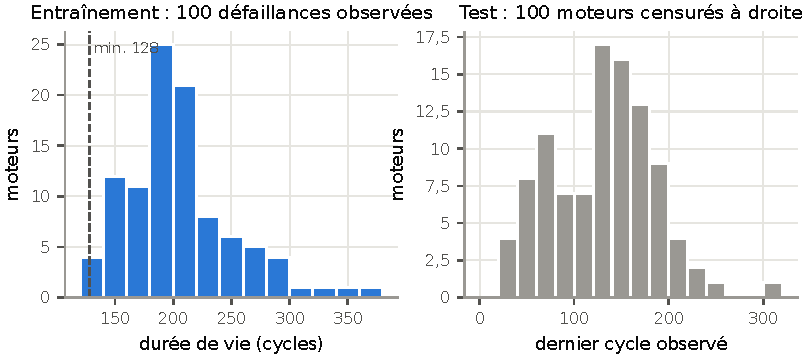
\includegraphics[width=1\linewidth]{figures/donnees_durees_de_vie.pdf}
\caption{Durées de vie des moteurs d'entraînement (gauche) et durées observées, censurées à droite, des moteurs de test (droite).}\label{fig:donnees_durees_de_vie}
\end{figure}

\subsection{Capteurs constants}\label{sec:donnees-capteurs}

Avec une seule condition opératoire, 7 capteurs prennent moins de 10 valeurs distinctes et sont écartés (s1, s5, s6, s10, s16, s18, s19), de même que les réglages opérationnels. Les autres capteurs dérivent progressivement au cours de la vie, avec un bruit important d'un cycle à l'autre, d'où l'usage de moyennes glissantes.

\chapconclusion

Ce chapitre a fixé le cadre et les méthodes de référence de l'étude. Le jeu FD001 fournit 200 unités pour la fiabilité, dont 100 censurées, sans défaillance avant 128 cycles. Le chapitre suivant présente les méthodes appliquées à ces données.
